\documentclass[12pt]{article}

\usepackage[a4paper,left=3cm,top=3cm,right=2cm,bottom=2cm]{geometry}

\usepackage[utf8]{inputenc}
\usepackage[T1]{fontenc}
\usepackage[brazil]{babel}
\usepackage{newtxtext,newtxmath}
\usepackage{indentfirst}
\usepackage{setspace}
\usepackage{titlesec}
\usepackage{graphicx}
\usepackage{float}
\usepackage{enumitem}
\usepackage{hyperref}

\usepackage{fancyhdr}
\pagestyle{fancy}
\renewcommand{\headrulewidth}{0pt}
\fancyhf{}
\fancyhead[rh]{\thepage}
\fancypagestyle{plain}{
  \renewcommand{\headrulewidth}{0pt}
  \fancyhf{}
  \fancyhead[rh]{\thepage}
}
\setlength{\headheight}{15pt}

\makeatletter
\def\verbatim@font{\small\ttfamily}
\makeatother

% Configuracoes ABNT %
\onehalfspacing{}
\setlength{\parskip}{6pt}
\setlength{\parindent}{1.5cm}
\titlespacing{\section}{0pt}{12pt plus 4pt minus 4pt}{12pt plus 4pt minus 4pt}

\begin{document}

\title{Guia Rápido para Conexão com o Servidor do LaR}

\author{Laboratório de Robótica da UFBA}

\date{2021}

\maketitle

\setcounter{page}{1} % needed if pages are to be continuously numbered

\section{Conexão com o Servidor}
A conexão do usuário com o servidor do LaR deve ser feita através da VPN da UFBA, e ele precisará também de credenciais a serem passadas pelo professor responsável.
Atendidos os requisitos, a conexão pode ser feita pelos seguintes passos:

\begin{enumerate}[font=\bfseries]
    \item Acesse o site do LaR pelo endereço \url{http://10.131.16.32/}, clique no menu Acesso e no submenu Servidor, para ir à tela de login da plataforma Guacamole.
    
    \begin{figure}[H]
    \centering
    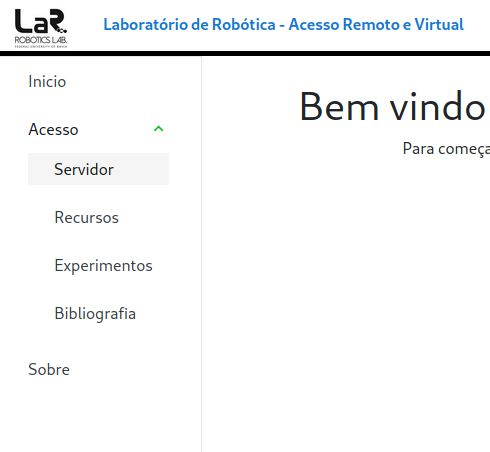
\includegraphics[width=0.6\textwidth]{img/site-lar.jpg}
    \caption{\label{ref:site-lar}Acesso ao servidor remoto pelo site do LaR.}
    \end{figure}
    
    \pagebreak
    
    \item Após entrar com suas credenciais e ser direcionado à tela de seleção de usuário, acesse a conexão destinada à sua demanda (\verb|experimentos|, por exemplo)*.
    
    \subparagraph{*OBS.} A conexão \verb|alunoXX| com mesmo número que seu usuário é uma conexão dedicada que guarda seu estado de uso mesmo após desconexões, mas precisa ser ativada de antemão pelo administrador do sistema.
    Para uso geral, a \verb|aluno-geral| cria conexões temporárias sob demanda.
    A conexão \verb|experimentos| é dedicada, tem acesso aos equipamentos disponíveis no laboratório e a princípio aberta a todos os usuários, porém comporta apena uma conexão por vez.
    
    \begin{figure}[H]
    \centering
    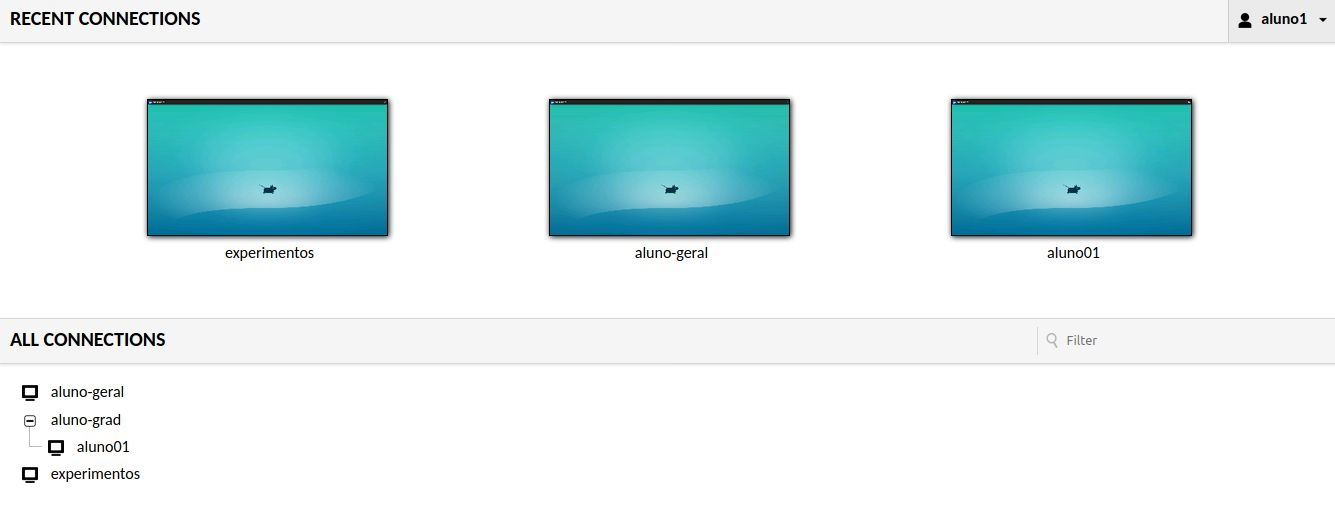
\includegraphics[width=0.9\textwidth]{img/conexao-guaca.jpg}
    \caption{\label{ref:conexao-guaca}Tela de conexões do Guacamole.}
    \end{figure}
    
    \item Os aplicativos disponíveis ao usuário, mais especificamente o Painel de Controle Virtual da DE2-115, podem ser acessados pelo launcher \textit{Applications} do ambiente virtual, no canto superior esquerdo do desktop.
    
    \begin{figure}[H]
    \centering
    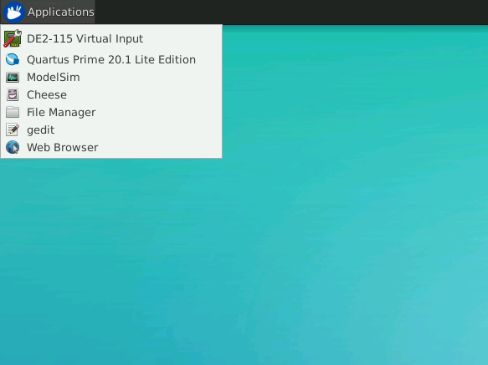
\includegraphics[width=0.6\textwidth]{img/launcher-experimentos.jpg}
    \caption{\label{ref:launcher}Aplicativos disponíveis.}
    \end{figure}
    
    \item O menu da sessão Guacamole pode ser acessado com a combinação Ctrl+Shift+Alt, e é por ele que podem ser feitas configurações de input, transferência de arquivos, logout, entre outras.
    
    \item É possível compartilhar a sessão com qualquer pessoa com acesso à VPN da UFBA clicando no botão \textit{Share} na parte superior do menu da sessão. O convite pode ser feito apenas para visualização ou com privilégios de edição.
    
    \begin{figure}[H]
    \centering
    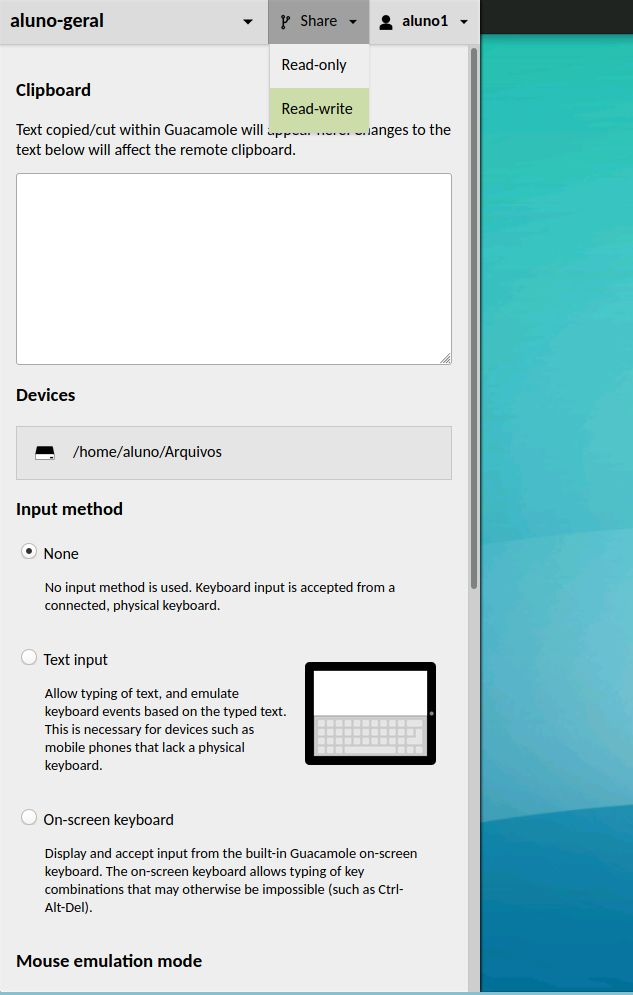
\includegraphics[width=0.6\textwidth]{img/share-guac.jpg}
    \caption{\label{ref:share-guac}Menu da sessão Guacamole com opções de compartilhamento.}
    \end{figure}
    
    \item Nos arquivos do usuário existe a pasta \verb|Arquivos| para a qual podem ser transferidos arquivos pessoais para uso remoto, assim como a operação contrária. Para isso basta abri-la pelo menu da sessão Guacamole em \textit{Devices}, onde aparecerão os arquivos presentes na pasta e um botão para upload. Para fazer download basta clicar duas vezes em um dos arquivos. Pastas terão que ser comprimidas antes de serem transferidas.
    
    \begin{figure}[H]
    \centering
    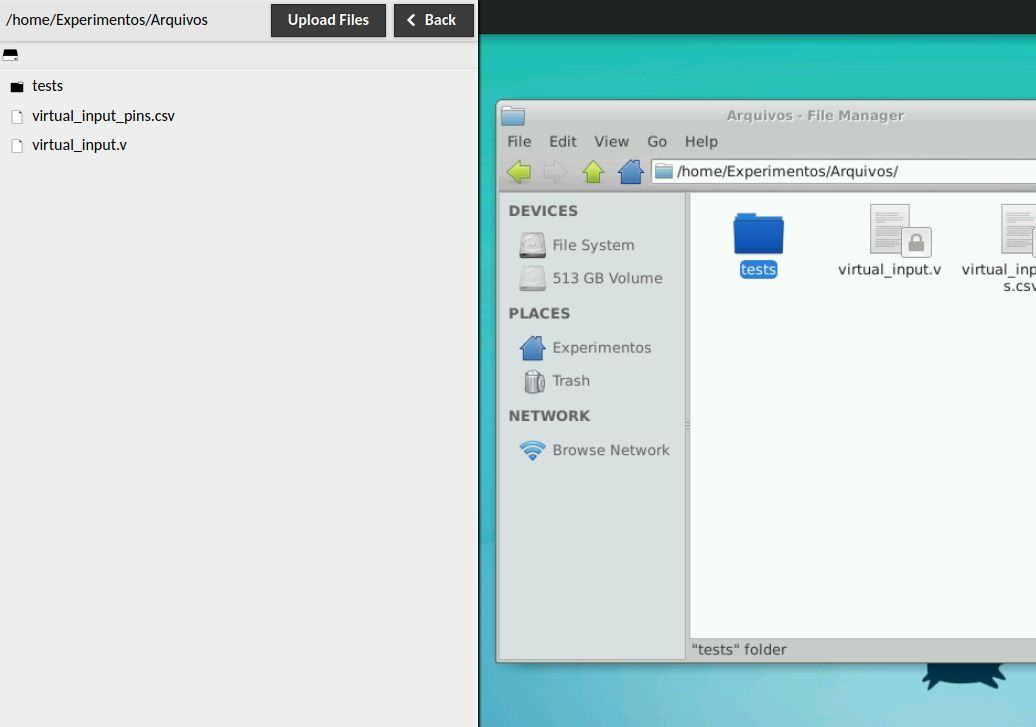
\includegraphics[width=0.8\textwidth]{img/trans-guaca.jpg}
    \caption{\label{ref:trans-guaca}Interface de transferência de arquivos pelo menu da sessão.}
    \end{figure}
    
    \item Para desconectar, basta clicar no botão com o nome do usuário no canto superior direito do menu da sessão Guacamole.
\end{enumerate}

\end{document}
